\documentclass[a4paper, man, floatsintext]{apa6}
\usepackage{lmodern}
\usepackage{amssymb,amsmath}
\usepackage{ifxetex,ifluatex}
\usepackage{fixltx2e} % provides \textsubscript
\ifnum 0\ifxetex 1\fi\ifluatex 1\fi=0 % if pdftex
  \usepackage[T1]{fontenc}
  \usepackage[utf8]{inputenc}
\else % if luatex or xelatex
  \ifxetex
    \usepackage{mathspec}
  \else
    \usepackage{fontspec}
  \fi
  \defaultfontfeatures{Ligatures=TeX,Scale=MatchLowercase}
\fi
% use upquote if available, for straight quotes in verbatim environments
\IfFileExists{upquote.sty}{\usepackage{upquote}}{}
% use microtype if available
\IfFileExists{microtype.sty}{%
\usepackage{microtype}
\UseMicrotypeSet[protrusion]{basicmath} % disable protrusion for tt fonts
}{}
\usepackage{hyperref}
\hypersetup{unicode=true,
            pdfauthor={Jana B. Jarecki},
            pdfborder={0 0 0},
            breaklinks=true}
\urlstyle{same}  % don't use monospace font for urls
\usepackage{graphicx,grffile}
\makeatletter
\def\maxwidth{\ifdim\Gin@nat@width>\linewidth\linewidth\else\Gin@nat@width\fi}
\def\maxheight{\ifdim\Gin@nat@height>\textheight\textheight\else\Gin@nat@height\fi}
\makeatother
% Scale images if necessary, so that they will not overflow the page
% margins by default, and it is still possible to overwrite the defaults
% using explicit options in \includegraphics[width, height, ...]{}
\setkeys{Gin}{width=\maxwidth,height=\maxheight,keepaspectratio}
\IfFileExists{parskip.sty}{%
\usepackage{parskip}
}{% else
\setlength{\parindent}{0pt}
\setlength{\parskip}{6pt plus 2pt minus 1pt}
}
\setlength{\emergencystretch}{3em}  % prevent overfull lines
\providecommand{\tightlist}{%
  \setlength{\itemsep}{0pt}\setlength{\parskip}{0pt}}
\setcounter{secnumdepth}{0}
% Redefines (sub)paragraphs to behave more like sections
\ifx\paragraph\undefined\else
\let\oldparagraph\paragraph
\renewcommand{\paragraph}[1]{\oldparagraph{#1}\mbox{}}
\fi
\ifx\subparagraph\undefined\else
\let\oldsubparagraph\subparagraph
\renewcommand{\subparagraph}[1]{\oldsubparagraph{#1}\mbox{}}
\fi

%%% Use protect on footnotes to avoid problems with footnotes in titles
\let\rmarkdownfootnote\footnote%
\def\footnote{\protect\rmarkdownfootnote}

%%% Change title format to be more compact
\usepackage{titling}

% Create subtitle command for use in maketitle
\providecommand{\subtitle}[1]{
  \posttitle{
    \begin{center}\large#1\end{center}
    }
}

\setlength{\droptitle}{-2em}

  \title{}
    \pretitle{\vspace{\droptitle}}
  \posttitle{}
    \author{Jana B. Jarecki}
    \preauthor{\centering\large\emph}
  \postauthor{\par}
      \predate{\centering\large\emph}
  \postdate{\par}
    \date{02 Oktober, 2019}

\usepackage{natbib} \usepackage{threeparttable} \usepackage{booktabs}
\shorttitle{test} \usepackage{setspace}
\AtBeginEnvironment{tabular}{\singlespacing} \usepackage{times}
\usepackage{changes} \definechangesauthor[name={JJ}, color=orange]{jj}
\usepackage{upgreek} \AtBeginDocument{\let\maketitle\relax}

\begin{document}

\subsection{Evaluations of Gambles by Condition and Sample Size}

Table \ref{tab:means_study1} shows participants' evaluations of the
gambles in the experience and description conditions. Notably, the
evaluations in the experience condition stay relatively constant across
sample sizes. In the best-fitting mixed regression model
\(\mathrm{M}\textsubscript{0}\) sample size was included as a random
effect, and gamble type---p-bet vs. \$-bet---as a fixed effect,
resulting in higher evaluations of the p-bets (gamble IDs 1 to 3)
compared to the \$-bets (IDs 4 to 6). This model outperformed a model
with sample size as fixed effect (\(BF\textsubscript{01} = 409\)), and a
model with a sample-size\(\times\)gamble-type interaction
(\(BF\textsubscript{01} > 1,000\)).

\begin{table}[tbp]
\begin{center}
\begin{threeparttable}
\caption{\label{tab:means_study1}Valuations of Gambles in Study 1}
\begin{tabular}{lccccrr}
\toprule
Condition & Sample size category & Effective sample size & \textit{Med} & \textit{M} & D--E & D--E:$BF\textsubscript{10}$\\
\midrule
Gamble ID 1 &  &  &  &  &  & \\
\ \ \ E & xs & 5 & 5.00 & 5.16 & -0.56 & 4\\
\ \ \ E & s & 10 & 4.55 & 5.30 & -0.70 & 60\\
\ \ \ E & m & 15 & 5.00 & 5.34 & -0.74 & 23\\
\ \ \ E & l & 30 & 5.00 & 5.29 & -0.69 & 147\\
\ \ \ D & -- & -- & 4.00 & 4.60 & -- & --\\
Gamble ID 2 &  &  &  &  &  & \\
\ \ \ E & xs & 6 & 4.00 & 4.33 & -0.71 & 134\\
\ \ \ E & s & 12 & 4.00 & 4.31 & -0.69 & 589\\
\ \ \ E & m & 18 & 4.00 & 4.04 & -0.43 & 5\\
\ \ \ E & l & 36 & 4.00 & 3.99 & -0.37 & 2\\
\ \ \ D & -- & -- & 3.00 & 3.61 & -- & --\\
Gamble ID 3 &  &  &  &  &  & \\
\ \ \ E & xs & 7 & 6.00 & 7.56 & -0.99 & 4\\
\ \ \ E & s & 14 & 6.70 & 8.40 & -1.83 & 902\\
\ \ \ E & m & 21 & 6.20 & 7.92 & -1.35 & 135\\
\ \ \ E & l & 42 & 6.00 & 7.68 & -1.11 & 23\\
\ \ \ D & -- & -- & 5.00 & 6.57 & -- & --\\
Gamble ID 4 &  &  &  &  &  & \\
\ \ \ E & xs & 5 & 3.00 & 2.80 & 0.28 & >1000\\
\ \ \ E & s & 10 & 3.20 & 2.91 & 0.16 & 3\\
\ \ \ E & m & 15 & 3.00 & 2.80 & 0.28 & 56\\
\ \ \ E & l & 30 & 3.00 & 2.95 & 0.13 & 1\\
\ \ \ D & -- & -- & 3.20 & 3.08 & -- & --\\
Gamble ID 5 &  &  &  &  &  & \\
\ \ \ E & xs & 6 & 2.00 & 1.77 & 0.10 & 8\\
\ \ \ E & s & 12 & 2.00 & 1.75 & 0.12 & 17\\
\ \ \ E & m & 18 & 2.00 & 1.73 & 0.14 & 28\\
\ \ \ E & l & 36 & 2.00 & 1.81 & 0.06 & 1\\
\ \ \ D & -- & -- & 2.00 & 1.87 & -- & --\\
Gamble ID 6 &  &  &  &  &  & \\
\ \ \ E & xs & 7 & 4.00 & 3.46 & 0.18 & 3\\
\ \ \ E & s & 14 & 4.00 & 3.55 & 0.09 & 0\\
\ \ \ E & m & 21 & 4.00 & 3.58 & 0.06 & 0\\
\ \ \ E & l & 42 & 4.00 & 3.70 & -0.06 & 0\\
\ \ \ D & -- & -- & 4.00 & 3.64 & -- & --\\
\bottomrule
\addlinespace
\end{tabular}
\begin{tablenotes}[para]
\normalsize{\textit{Note.} \textit{M} = mean, \textit{Med} = median, D--E = difference between mean description-based valuations and experience-based valuations, $BF\textsubscript{10}$ = Bayes Factor quantifying the evidence for a linear model $\mathrm{M}\textsubscript{1}$ predicting that valuations differ between description and experience over a linear model $\mathrm{M}\textsubscript{0}$ predicting no such differences; both models models contain a by-participant random effect. Gambles IDs 1, 2, and 3 are \$-bets; Gamble IDs 4, 5, and 6 are p-bets.}
\end{tablenotes}
\end{threeparttable}
\end{center}
\end{table}

\subsection{Cognitive Modeling of Experience-based Evaluations by Sample Size}

To unpack the role of sample size in value judgments more closely, we
used cognitive computational modeling. We compared the performance of
the \added[id=jj]{relative frequency} (RF) model and the
\added[id=jj]{Bayesian value updating} (BVU) model regarding the
observed evaluations.
\added{The models were compared to a baseline model, predicting a constant evaluation equal to the mean  individual evaluation (sensible models are expected to outperform this baseline model).}

\subsubsection{Modeling Procedure}

\added[id=jj]{The observed and predicted evaluations were normalized to a common range (0 - 1, by division through the gain magnitude and truncation of normalized values $>$ 1). The free model parameters were estimated by maximum likelihood at the participant level, assuming observations follow a truncated normal distribution, censored at 0 and 1, around the model predictions with a constant standard deviation ($\sigma$) estimated as a free parameter ($0 < \sigma \leq 1$).  Therefore, the relative frequency model had 2 free parameter, the power utility exponent $\alpha$ ($0 \leq \alpha \leq 20$) and $\sigma$. The Bayesian value updating model had 4 free parameter the gain prior $\theta_G$ ($0 \leq \theta_G \leq 1$; the loss prior was $\theta_0=2-\theta_G$), the learning rate $\delta$ ($0 \leq \delta \leq 10$), $\alpha$ and $\sigma$. A 3-parameter Bayesian value updating model was also tested, which had a fixed learning rate of $\delta=1$ (optimal Bayesian updating). The baseline model had 2 free parameter, the mean evaluation $\mu$ and $\sigma$. We estimated the parameters with a local solver using a augmented Lagrange multiplier method \citep[Rsolnp package, version 1.16]{Ghalanos2015}. We compared the models by the Bayesian information criterion (BIC), transformed into Bayesian evidence weights \citep[][1 means very strong evidence for a competitor model]{Kass1995, Lewandowsky2011}}.

\subsubsection{Modeling Results}
\added[id=jj]{We will first outline the quantitative model fit, followed by the qualitative model fit, and lastly analyze the effects of sample size given the cognitive strategies.}
\subsubsection{Quantitative Model Fit.}

The Bayesian value updating model described about half of the
participants best (30 of 40; 75\%), and the relative frequency model
described a minority of participants (9; 22\%). The baseline model
described NA participants best. Figure \ref{fig:model_weights} shows the
evidence strength for the models by participant. The models' mean
Bayesian information criterion across all participants equaled
BIC\textsubscript{BVU}\(=\) -124, BIC\textsubscript{RF}\(=\) -110, and
BIC\textsubscript{BASE}\(=\) NA.

\begin{figure}

{\centering 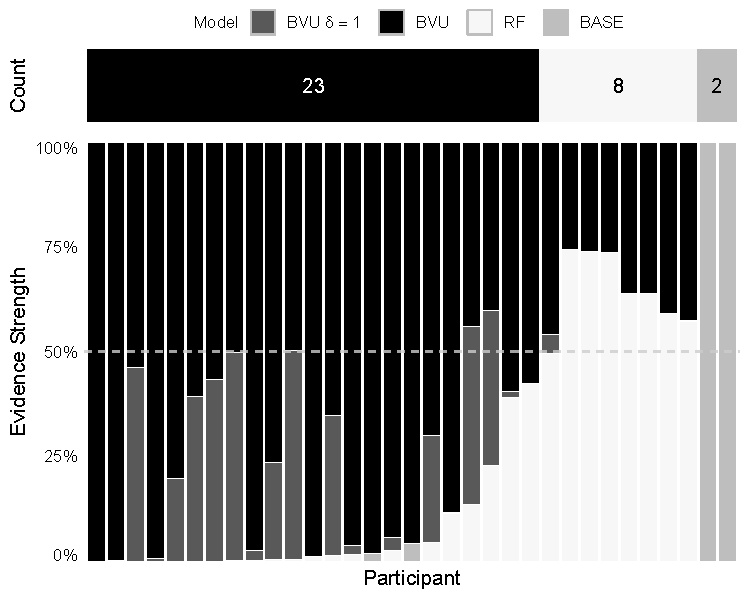
\includegraphics{../figures/model_weights-1} 

}

\caption{Evidence for the models for individual participants. \textit{RF}$=$ relative frequency model, \textit{BVU}$=$ Bayesian value updating model, \textit{BASE}$=$ Baseline model.}\label{fig:model_weights}
\end{figure}

The estimated parameter of the winning models, which Table
\ref{tab:model_par} summarizes, reveal that the power utility exponent
(\(\alpha\)) is almost identical for the participants using a Bayesian
value updating strategy (\(M_{\alpha}= 1.433\)) and those using a
relative frequency strategy (\(M_{\alpha}=1.598\)) . Participants using
the Bayesian strategy had a prior belief that gains are less likely
(B\textsubscript{BVU,0}=46.078\%) than zero outcomes (gain prior
\(\theta_G = 0.922; zero-outcome prior \theta_0 = 1.078\)). Their
estimated learning rate \(\delta\) was anti-conservative
(\(M_{\delta}=1.362\), values \(<\) 1 mean conservative, 1 is optimal
Bayesian, \(>\) 1 is liberal learning), which is contrary to other
findings indicate conservative Bayesian learners
\citep{Edwards1967,Tauber2017}. The reason for their liberal learning
may be the repeated exposure to the same gambles.

\begin{table}[tbp]
\begin{center}
\begin{threeparttable}
\caption{\label{tab:model_par}Parameter Estimates of Winning Models, \textit{M (SD)}}
\begin{tabular}{lccccc}
\toprule
Winning Model & $\alpha$ & $\delta$ & $\theta_G$ & $\mu$ & $\sigma$\\
\midrule
BASE & -- & -- & -- & 0.47 (NA) & 0.30 (NA)\\
RF & 1.61 (0.58) & -- & -- & -- & 0.12 (0.02)\\
BVU & 1.49 (1.47) & 1.36 (2.12) & 0.92 (0.66) & -- & 0.13 (0.07)\\
\bottomrule
\addlinespace
\end{tabular}
\begin{tablenotes}[para]
\normalsize{\textit{Note.} \textit{BVU}$=$ Bayesian value updating model, \textit{RF}$=$ relative frequency model, \textit{BASE}$=$baseline model. Parameters denote: $\alpha=$ power utility exponent, $\theta_G$ gain prior, $\mu=$ mean evaluation, $\sigma$ standard deviation.}
\end{tablenotes}
\end{threeparttable}
\end{center}
\end{table}
\subsubsection{Qualitative Model Fit.}
\added[id==jj]{The qualitative fit between the models and the data can be examined by plotting observed evaluations against the predicted evaluations, where predictions stem from the respective participant's best-fitting model with optimized parameters. Figure \ref{fig:ind_fits1} shows that the models generally capture the data well, except in four cases, where even the winning model fails to resemble the data. For participants number 1, 19, 24, and 38, for whom the winning model is the Bayesian updating (BVU) model, even the Bayesian model must be rejected because it mis-fits the data qualitatively.}

\begin{figure}

{\centering 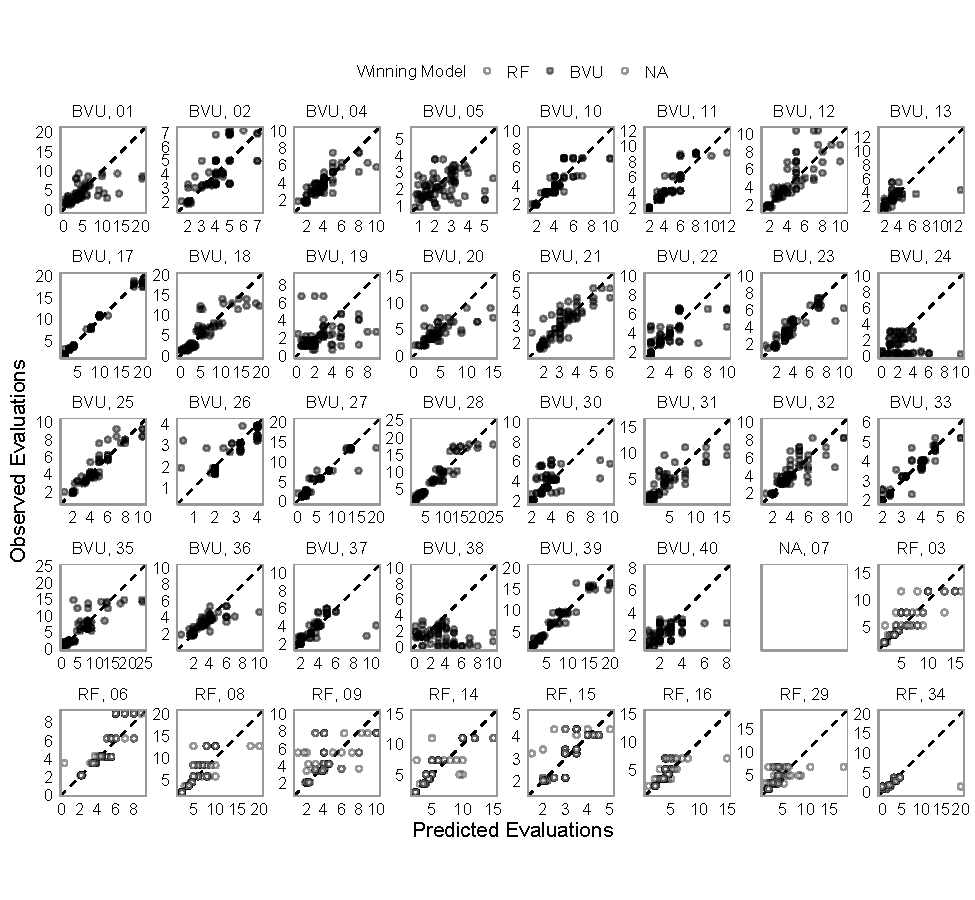
\includegraphics{../figures/ind_fits1-1} 

}

\caption{Predicted evaluations from the best-fitting models plotted against the observed evaluations (by participant). \textit{BVU}$=$ Bayesian value updating model, \textit{RF}$=$ relative frequency model, \textit{BASE}$=$baseline model.}\label{fig:ind_fits1}
\end{figure}

\added{The heterogeneity in strategies that resulted from the cognitive modeling helps interpreting the null finding---that sample size has no effect on evaluations---that we observed at the aggregate level (Table \ref{tab:means_study1}). The aggregate analysis fails to take the individual differences in strategy use into account. The distribution of winning model indicates that our sample is best described by a mixture of strategies, which the aggregate analyses could not pick up. Moreover, the aggregate analysis fails to account for the prior beliefs regarding gain probabilities. Depending on the prior belief, the Bayesian value updating (BVU) model predicts either a decrease or an increase in valuations with increasing sample size.}

\emph{The effect of sample size given cognitive strategies.} Next, we
qualitatively analyzed if sample size differentially affects the
relative-frequency-type and Bayesian-type learners. We expected that
sample size changes evaluations of the Bayesian learners depending on
their priors, but that sample size does not change the evaluations of
the frequency-type learners.

\begin{figure}

{\centering 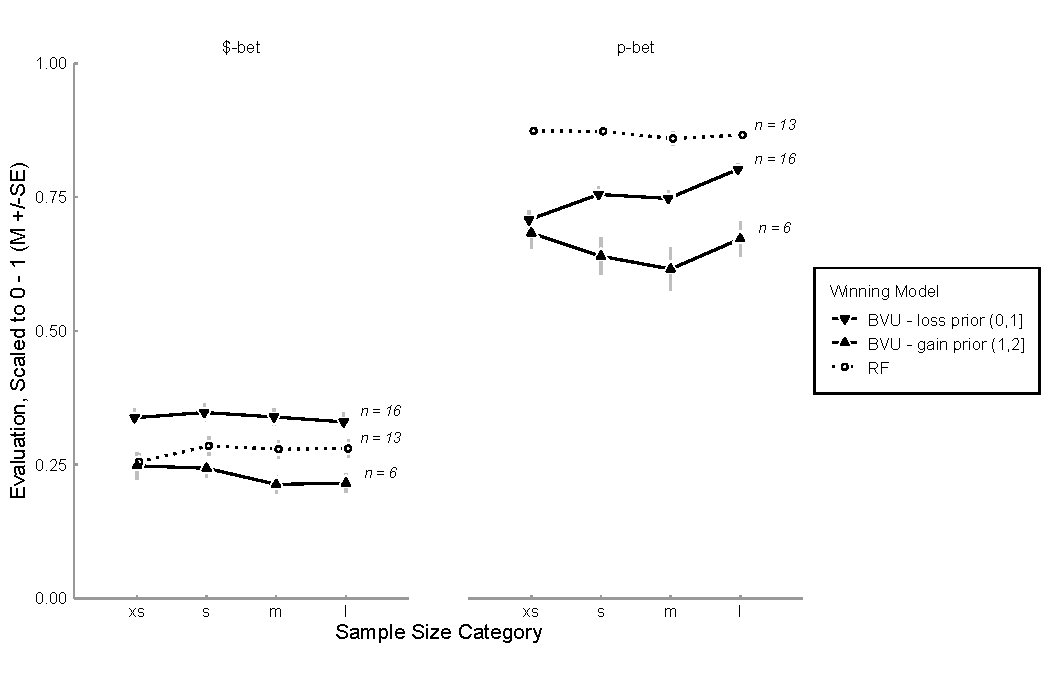
\includegraphics{../figures/qual1-1} 

}

\caption{Mean evaluation (standardized to 0 - 1) split by winning model and prior beliefs of the BVU model. \textit{BVU}$=$Bayesian value updating model, \textit{RF}$=$ Relative frequency model. Error bars indicate standard errors. \textit{\$-bet}: low-probability high-outcome gambles, \textit{p-bet}: high-probability low-outcome gambles. Sample sizes (xs, x, m, l), see Table \ref{tab:Lotteries}. \textit{n=16, 13, 6} denotes the number of participants best-described by the respective models.}\label{fig:qual1}
\end{figure}

\added[id=jj]{
Our next analysis examines the interaction between the cognitive strategies and the number of samples that participants drew. Whereas the relative-frequency model holds that higher sample sizes should not affect the evaluation of the gambles, the Bayesian model predicts that sample size changes in the evaluations and that the changes depend on the prior beliefs and the environment. A gain prior---initially believing that gains are more likely than zero-outcomes---should decrease the valuations as sample sizes increase, but only for \$-bets, where gains are in fact less likely (14 to 20\%) than zero-outcomes (Table~\ref{table:Lotteries}). By contrast, a zero-outcome prior---initially believing that zero-outcomes are more likely than gains---should increase the valuations with higher sample sizes for p-bets, where in fact gains are more likely (80 to 86\%) than zero-outcomes (Table~\ref{table:Lotteries}).
}

\added[id=jj]{
Participants were classified based on the best-fitting model into relative-frequency learners, Bayesian learners with gain priors (parameter $\theta_G > 1$), and Bayesian learners with loss priors (parameter $\theta_G \leq 1$). Figure \ref{fig:qual1} shows the observed change in evaluations with sample size, separately for p-bets and \$-bets. The relative-frequency learners evaluated both p-bets and \$-bets relatively constantly across sample sizes, whereas the Bayesian learners increased their evaluations if they started with a loss prior and decreased their evaluations after starting with a gain prior, at least for p-bets (high-gain low-probability gambles). The Bayesian learners were relatively constant in their evaluations of \$-bets across sample sizes.
}

\added[id=jj]{
A Bayesian generalized linear model of the (normalized) evaluations of gambles as a function of sample size, gamble type (p-bet, \$-bet), and best-fitting cognitive model with a by-participant random intercept confirmed the expectations. Participants classified as Bayesian with gain priors decreased their evaluation of \$-bets by about 2\% as sample size increased, trend $-0.020$, 95\% HPD [$-0.034, -0.004$]. Also as expected, participants that were best-described by relative-frequency strategy did not change their \$-bet evaluations with sample size (trend $0.011$, 95\% HPD $[-0.004, 0.027]$), and neither did Bayesian participants with loss priors (trend $-0.000$, 95\% HPD $[-0.011, 0.011]$). Regarding p-bets, participants that were best-described by a Bayesian model with loss priors increased their evaluation by about 2\% with increasing sample size, as expected (trend $0.024$, 95\% HPD $[0.014, 0.036]$); participants with gain priors decreased their p-bet evaluations with sample size (trend $-0.003$, 95\% HPD $[-0.017, 0.013]$). Also as expected, the relative-frequency participants did not change their p-bet evaluations with sample size $-0.005$, 95\% HPD $[-0.021, 0.010]$.

}


\end{document}
